\documentclass[12pt]{article}
\usepackage{geometry}
\geometry{letterpaper, left=22.5mm, right=22.5mm, top=30mm, bottom=30mm}
\geometry{letterpaper}
\usepackage{amsmath}
\usepackage{amssymb}
\usepackage{enumitem}
\usepackage{fancyhdr}
\usepackage{framed}
\usepackage{tikz}
\usepackage{mathpazo}
%\usepackage{charter}
%\usepackage{newcent}
\usepackage{indentfirst}
\usepackage{booktabs}
\usepackage{graphicx}
\usepackage{float}
\usepackage{makecell}
\usepackage{xcolor}
\usepackage{mdframed}
\usetikzlibrary{trees}
\pagestyle{fancy}
\usepackage{amsthm}
\theoremstyle{definition}
\newtheorem{definition}{Definition}[section]
\theoremstyle{property}
\newtheorem{property}{Property}[section]
\theoremstyle{assumption}
\newtheorem{assumption}{Assumption}[section]
\theoremstyle{example}
\newtheorem{example}{Example}[section]
\theoremstyle{comment}
\newtheorem{comment}{Comment}[section]
\newtheorem{theorem}{Theorem}[section]
\newtheorem{corollary}{Corollary}[theorem]
\newtheorem{lemma}[theorem]{Lemma}
\usepackage{lastpage}
\usepackage{wrapfig}
\usepackage{hyperref}
\usepackage{subcaption}
\usepackage{setspace}
\hypersetup{
colorlinks=true,
linkcolor=black,
filecolor=green, 
urlcolor=blue,
}
\newcommand{\ROM}[1]
    {\MakeUppercase{\romannumeral #1}}
\fancyhead[L]{Econometrics: Recitation 1}%change each reci
\fancyhead[R]{Fall2022}
\fancyfoot[C]{\thepage \hspace{1pt} / \pageref{LastPage}}

\fancypagestyle{firstpage}{%
\fancyhf{}%
\renewcommand{\headrulewidth}{0mm}%
  \fancyfoot[C]{\thepage \hspace{1pt} / \pageref{LastPage}}
}
%change title each rec
\title{Introduction to Econometrics: Recitation 3}

\begin{document}
\linespread{1.25}
\onehalfspacing

\author{Seung-hun Lee\footnote{Contact me at \href{mailto:sl4436@columbia.edu}{sl4436@columbia.edu} if you spot any errors or have suggestions on improving this note.}}
\date{September 29th, 2022}
\maketitle
\thispagestyle{firstpage}

%%%%%%%%%%%%%%%%%%

\section{Ordinary least squares}

\subsection{Main Assumptions of the OLS Estimators}
For the ordinary least squares to have desired properties of unbiasednesss, consistency, efficiency, and asymptotic normality, the following assumptions must be made
\begin{mdframed}[backgroundcolor=blue!5] 
\begin{assumption} Here are the assumptions for the classical linear regression model
\begin{itemize}
\item[\textbf{A0}] Linearity: The regression is assumed to be linear in parameters.
\[
\text{Okay: } Y_i = \beta_0 + \beta_1X_i + \beta_2X_i^2+u_i 
\]
\[
\text{Not: } Y_i = \beta_0 + \beta_1X_i + \beta_2^2X_i+u_i,
\]
\item[\textbf{A1}] $E(u_i|X_i)=0$: This means that conditional on letting $X_i$ take a certain value, we are not making any systematical error in the linear regression. This is required for the OLS to be unbiased. (Alternately, you can say $cov(X_i,u_i)=0$, an exogeneity condition.)
\item[\textbf{A2}] i.i.d. (random sampling): $(X_i,Y_i)$ is assumed to be from independent, identical distribution
\item[\textbf{A3}] No Outliers: Outlier has no impact on the regression results. ($E(X_i^4), E(Y_i^4)<\infty$)
\item[\textbf{A4}] Homoskedasticity: $var(u_i)=\sigma_2$, or variance of $u_i$ does not depend on $X_i$. If this condition is broken, there exists a \textit{heteroskedasticity}
\item[\textbf{A5}] No Autocorrelation (Serial Correlation): For $i\neq j$, $cov(u_i,u_j)=0$. In other words, error at the previous period does not have any impact on the current period. This is usually broken in time series settings, where the error in the previous period carries over to the next period.
\end{itemize}
\end{assumption}
\end{mdframed}

\subsection{Sampling distribution of OLS}
Note that the OLS estimate that we are getting is a random variable - the estimate we get is different depending on which sample we work with. This is why we can discuss the distributional properties - mean and variance, in particular - of the OLS. 
\begin{itemize}
\item $\hat{\beta}_1$: Recall that we can write
\[
\hat{\beta}_1= \frac{\sum_{i=1}^n(X_i-\bar{X})(Y_i-\bar{Y})}{\sum_{i=1}^n(X_i-\bar{X})^2}
\]
Now, replace $Y_i$ an $\bar{Y}$ with 
\[
Y_i =\beta_0 + \beta X_i + u_i, \ \bar{Y} = \beta_0 + \beta_1\bar{X} + \bar{u},
\]
which allows us to write 
\[
(Y_i-\bar{Y}) = (\beta_1(X_i-\bar{X})+(u_i-\bar{u}))
\]
and get
\[
\hat{\beta}_1=\beta_1+  \frac{\sum_{i=1}^n(X_i-\bar{X})(u_i-\bar{u})}{\sum_{i=1}^n(X_i-\bar{X})^2}
\]
We are now ready to discuss the distributional properties
\begin{itemize}
\item $E[\hat{\beta}_1]$: It can be written as
\[
\begin{aligned}
E[\hat{\beta}_1]& = E\left[\beta_1+  \frac{\sum_{i=1}^n(X_i-\bar{X})(u_i-\bar{u})}{\sum_{i=1}^n(X_i-\bar{X})^2}\right]\\
&=\beta_1+ E\left[\frac{\sum_{i=1}^n(X_i-\bar{X})(u_i-\bar{u})}{\sum_{i=1}^n(X_i-\bar{X})^2}\right]
\end{aligned}
\]
Note that the $\sum_{i=1}^n(X_i-\bar{X})(u_i-\bar{u})$ can be written to something simpler. This is equal to
\[
\sum_{i=1}^n(X_i-\bar{X})(u_i-\bar{u})=\sum_{i=1}^nX_iu_i-\bar{u}\sum_{i=1}^n X_i-\bar{X}\sum_{i=1}^nu_i+n\bar{X}\bar{u}
\]
Since $\bar{X}$ is a sample mean of $X$, $\sum_{i=1}^nX_i=n\bar{X}$. Thus, we get
\[
\sum_{i=1}^n(X_i-\bar{X})(u_i-\bar{u})=\sum_{i=1}^nX_iu_i-\bar{X}\sum_{i=1}^nu_i=\sum_{i=1}^n(X_i-\bar{X})u_i
\]
The assumption that conditional mean is zero and $(X_i, u_i)$ are uncorrelated means that the term on the left hand side is zero. Therefore, IF THE CLASSICAL ASSUMPTIONS ARE VALID, $E[\hat{\beta}_1]=\beta_1$.
\item $var[\hat{\beta}_1]$: We use the definition of the variances and the fact that the expected value of $\hat{\beta}_1$ is unbiased (at least for now) to get
\[
\begin{aligned}
var(\hat{\beta}_1)&=E\left[\left(\hat{\beta}_1-E[\hat{\beta}_1]\right)^2\right] \\
&=E\left[\left(\hat{\beta}_1-{\beta}_1\right)^2\right]\\
&=E\left[\left( \frac{\sum_{i=1}^n(X_i-\bar{X})(u_i-\bar{u})}{\sum_{i=1}^n(X_i-\bar{X})^2} \right)^2\right]\\
&=E\left[\left(  \frac{(X_1-\bar{X})(u_1-\bar{u})}{\sum_{i=1}^n(X_i-\bar{X})^2}+...+\frac{(X_n-\bar{X})(u_n-\bar{u})}{\sum_{i=1}^n(X_i-\bar{X})^2} \right)^2\right]\\
\end{aligned}
\]
At the moment, we are assuming homoskedasticity and no autocorrelation. Since $X_i$ is from the data\footnote{Here, I am taking a slightly different angle from class. In class, we take $X_i$ as purely random variable. In that version, you get results that looks like the ones from class. Key takeaways, however, remain the same} and $u_i$ is a random error term, we can take all the $X_i$ terms in and keep the $u_i$ terms in the expectation to get (i.i.d assumption is also useful here)
\[
\begin{aligned}
var(\hat{\beta}_1)&=\frac{\sum_{i=1}^n(X_i-\bar{X})^2E[(u_i-\bar{u})^2]}{[\sum_{i=1}^n(X_i-\bar{X})^2]^2}\\
&=\frac{\sum_{i=1}^n(X_i-\bar{X})^2\sigma_u^2}{[\sum_{i=1}^n(X_i-\bar{X})^2]^2} \ (\because E[(u_i-\bar{u})^2]=var(u_i))\\
&=\sigma_u^2\frac{\sum_{i=1}^n(X_i-\bar{X})^2}{[\sum_{i=1}^n(X_i-\bar{X})^2]^2} =\frac{\sigma_u^2}{\sum_{i=1}^n(X_i-\bar{X})^2}
\end{aligned}
\]
Note that  to decrease the variance in the estimates, the variance of the error should be small relative to the variation in the $X_i$. Moreover, as the number of observations increase, the variance decreases through increase in the denominator.
\end{itemize}
At the end of the day, we can say the following about the distribution of our $\hat{\beta}_1$ estimator and use this to test our hypothesis
\[
\hat{\beta}_1 \sim N\left(\beta_1, \frac{\sigma_u^2}{\sum_{i=1}^n(X_i-\bar{X})^2}\right)
\]
\item $\hat{\beta}_0$: The formula for $\hat{\beta}_0$ is $\bar{Y}-\hat{\beta}_1\bar{X}$. By changing $\bar{Y}$, we can get
\[
\begin{aligned}
\hat{\beta}_0&=(\beta_0+\beta_1\bar{X}+\bar{u})-\hat{\beta}_1\bar{X}\\
&=\beta_0+(\beta_1-\hat{\beta}_1)\bar{X}+\bar{u}
\end{aligned}
\]
Then we can say the following about the sampling distribution
\begin{itemize}
\item $E[\hat{\beta}_0]$: We can write
\[
E[\hat{\beta}_0]=\beta_0+E[(\beta_1-\hat{\beta}_1)\bar{X}]+E[\bar{u}]=\beta_0
\]
since $\hat{\beta}_1$ is unbiased and conditional expectation of $u_i$ is zero. Thus, under our current assumptions, $\hat{\beta}_0$ is unbiased. 
\item $var[\hat{\beta}_0]$: Using the definition of the variance, we can write \[
\begin{aligned}
var(\hat{\beta}_0)&=E\left[\left(\hat{\beta}_0-E[\hat{\beta}_0]\right)^2\right] \\
&=E\left[\left(\hat{\beta}_0-{\beta}_0\right)^2\right]\\
&=E\left[\left( (\beta_1-\hat{\beta}_1)\bar{X}+\bar{u}\right)^2\right]\\
&=\bar{X}^2E\left[\left(\beta_1-\hat{\beta}_1 \right)^2\right]+ 2\bar{X}E\left[\left(\beta_1-\hat{\beta}_1 \right)\bar{u}\right] + E[\bar{u}^2]
\end{aligned}
\]
Under the assumption (A2), we can ignore the middle term as this is zero. The rest of the terms are $\bar{X}^2 var(\hat{\beta}_1)$ and $\frac{\sigma_u^2}{n}$. the final result is
\[
var(\hat{\beta}_0)=\frac{\sigma_u^2\bar{X}^2}{\sum_{i=1}^n(X_i-\bar{X})^2}+\frac{\sigma_u^2}{n}= \frac{\sigma_u^2}{n}\frac{\sum_{i=1}^nX_i^2}{\sum_{i=1}^n(X_i-\bar{X})^2}
\]
\end{itemize}
So we can write 
\[
\hat{\beta}_0 \sim N\left(\beta_0, \frac{\sigma_u^2}{n}\frac{\sum_{i=1}^nX_i^2}{\sum_{i=1}^n(X_i-\bar{X})^2}\right)
\]
\end{itemize}


\subsection{Measure of Fitness}
These numbers tell us how informative the sample linear regression we used is in telling us about the population data. In other words, they tell us how closely does our sample regression capture the data. We discussed three types of measure
\begin{itemize}
\item $\mathbf{R^2}$: It is defined as a fraction of total variation which is explained by the model. Mathematically, this is
\begin{gather*}
Y_i = \underbrace{\hat{\beta}_0 + \hat{\beta}_1X_i}_{\hat{Y}_i} + u_i, \ \bar{Y} = \underbrace{\hat{\beta}_0 + \hat{\beta}_1\bar{X}}_{\bar{\hat{Y}}} + \bar{u}, \\
\implies Y_i-\bar{Y} = (\hat{Y}_i - \bar{\hat{Y}}) - (u_i - \bar{u}) \\
\implies \sum_{i=1}^n (Y_i-\bar{Y})^2= \sum_{i=1}^n (\hat{Y}_i - \bar{\hat{Y}})^2+\sum_{i=1}^n(u_i - \bar{u})^2 - 2\sum_{i=1}^n(\hat{Y}_i - \bar{\hat{Y}}) (u_i - \bar{u})
\end{gather*}
Note that $\sum_{i=1}^n(\hat{Y}_i - \bar{\hat{Y}}) (u_i - \bar{u})=\sum_{i=1}^n\hat{Y}_i{u}_i-\bar{\hat{Y}}\sum_{i=1}^nu_i -\bar{u}\sum_{i=1}^n\hat{Y}_i +n\bar{u}\bar{\hat{Y}}$. Since $\sum_{i=1}^nu_i = n\bar{u},\ \sum_{i=1}^n\hat{Y}_i = n\bar{\hat{Y}}$ and $\sum_{i=1}^n\hat{Y}_iu_i=n\bar{u}\bar{\hat{Y}}$, all the terms cancel each other out. So we are left with
\[
\underbrace{\sum_{i=1}^n (Y_i-\bar{Y})^2}_{TSS}= \underbrace{\sum_{i=1}^n (\hat{Y}_i - \bar{\hat{Y}})^2}_{ESS}+\underbrace{\sum_{i=1}^n(u_i - \bar{u})^2}_{RSS} \implies 1=\frac{\sum_{i=1}^n (\hat{Y}_i - \bar{\hat{Y}})^2}{\sum_{i=1}^n (Y_i-\bar{Y})^2} + \frac{\sum_{i=1}^n(u_i - \bar{u})^2 }{\sum_{i=1}^n (Y_i-\bar{Y})^2}
\]
Thus, the $R^2$ can be found as
\[
R^2 = \frac{\sum_{i=1}^n (\hat{Y}_i - \bar{\hat{Y}})^2}{\sum_{i=1}^n (Y_i-\bar{Y})^2} = \frac{ESS}{TSS} = 1-\frac{RSS}{TSS}
\]
Intuitively, higher $R^2$ implies that the model explains more of the total variance, which implies that the regression fits the data well. 
\item $\mathbf{SER}$: Standard Error of Regression. It estimate the standard deviation of the error term in $Y_i$, or mathematically
\[
SER = \sqrt{\frac{1}{n-2}\sum_{i=1}^n u_i^2}
\]
where $u_i = y_i-\hat{y}_i$ and we use $n-2$ since there is loss of d.f. by two due to $\hat{\beta}_0, \hat{\beta}_1$. If SER turns out to be large, this implies that our model might be missing a key variable.

 \item \textbf{RMSE}: Root mean squared error. It is similar to SER in terms of how it looks, 
\[
RMSE = \sqrt{\frac{1}{n}\sum_{i=1}^n \hat{u}_i^2}
\]
this is used to assess the accuracy of the predictions. Numerically, the difference between SER and RMSE is minimal and even approximate to identical figure in large sample. 
\end{itemize}




\subsection{Hypothesis Tests}
We now have a sampling distribution for our OLS estimator. This now allows us to create a test statistic for the hypothesis test. In this note, we will talk about testing for the slope coefficient $\beta_1$. The idea is similar for our intercept $\beta_0$ and even if we have multiple $X_i$ variables. 
\begin{itemize}
\item\textbf{Test statistics} We know that the sampling distribution for $\hat{\beta}_1$ is
\[
\hat{\beta}_1 \sim N\left(\beta_1, \frac{\sigma_u^2}{\sum_{i=1}^n(X_i-\bar{X})^2}\right)
\]
To make the discussion simple, I now write $var(\hat{\beta}_1)=\frac{\sigma_u^2}{\sum_{i=1}^n(X_i-\bar{X})^2}$. There are two ways we go about this. One is where we know that actual value of $var(\hat{\beta}_1)$, through knowing $var(u_i)=\sigma_u$. The other case is where we do not know the exact value of $\sigma_u$ and are forced to estimate $var(u_i)$.
\item[$\to$] \textit{If we know $\sigma_u$}: This is a relatively easy case. Since the $\hat{\beta}_1$ takes a normal distribution, we can ``standardize" it to get the test statistic and the distribution for it. To do so, we simply subtract the mean from the estimate and divide the term by the standard deviation. That gets us
\[
\frac{\hat{\beta}_1-\beta_1}{\sqrt{var(\hat{\beta}_1)}}\sim N(0,1)
\]
Typically, the hypothesis test we use is (this is the default for the output tables in STATA)
\[
H_0: \beta_1=0 \ \ \text{vs} \ \ H_1: \beta_1\neq0
\]
Then, the test statistic becomes 
\[
t=\frac{\hat{\beta}_1}{\sqrt{var(\hat{\beta}_1)}}
\]
and you get to compare against the critical values that comes from the standard normal distribution. The critical values you use is determined by the significance level (5\% or 1\%), and the type of test you run (one vs two-tails).
\item[$\to$] \textit{If we don't know $\sigma_u$}: We are a bit unlucky in this case, but not by far. The difference is that you need to have an estimate for $var(\hat{\beta}_1)$ due to not knowing $\sigma_u$. The test statistics and its distribution is
\[
\frac{\hat{\beta}_1-\beta_1}{\sqrt{\widehat{var(\hat{\beta}_1)}}}\sim t_{n-2}
\]
where $\widehat{var(\hat{\beta}_1)}$ is the estimate for the variance and $t_{n-2}$ is a t-distribution with $n-2$ degrees of freedom. The degrees of freedom is determined by the number of observations, where 2 is subtracted because we are estimating $\beta_0$ and $\beta_1$ in the process. (\textit{Spoiler: In the multiple variable case with a constant and $k$ control variables, the degree of freedom is $n-k-1$}). Other than these differences, the idea that you need to compare with the appropriate critical value still carries over. \par\medskip
One comforting fact is that when $n$ is very large, t-distribution becomes very similar to the normal distribution. so the process of finding critical values are identical to the previous case.
\item \textbf{Confidence interval}: A 95\% confidence interval is a range of numbers that form a random interval that has a 95\% chance of including a (nonrandom) true value of a parameter. This can be obtained by inverting the rejection region that we have used in the critical value approach. \par\medskip
To make this simple, let's use a two-sided test  with 5\% significance level. as an example. Typically, the critical values are $\pm1.96$. We can tell that 
\[
\Pr\left(-1.96\leq \frac{\hat{\beta}_1-\beta_1}{\sqrt{var(\hat{\beta}_1)}} \leq1.96\right)=0.95
\]
We can switch around some terms to get $\beta_1$ in the middle, as a result
\[
\Pr\left(\hat{\beta}_1-1.96\times\sqrt{var(\hat{\beta}_1)} \leq \beta_1 \leq\hat{\beta}_1+1.96\times\sqrt{var(\hat{\beta}_1)}\right)=0.95
\]
In this way, we can find the upper and lower bounds of the confidence intervals. If they encompass the null test value - 0, for instance - then we cannot reject the null hypothesis. Otherwise, we can reject the null. 
\end{itemize}

\subsection{Heteroskedasticity}
We have assumed that the variance of the error term $var(u_i)$ is not a function of $X_i$. However, this assumption may not hold. In case where they do not hold, we can observe that the variance estimated under homoskedasticity assumption is (usually) underestimated. The graph on the left side is for the observations following the homoskedasticity assumption, while the one on the right does not follow homoskedasticity assumption.
\begin{figure}[H]
\centering
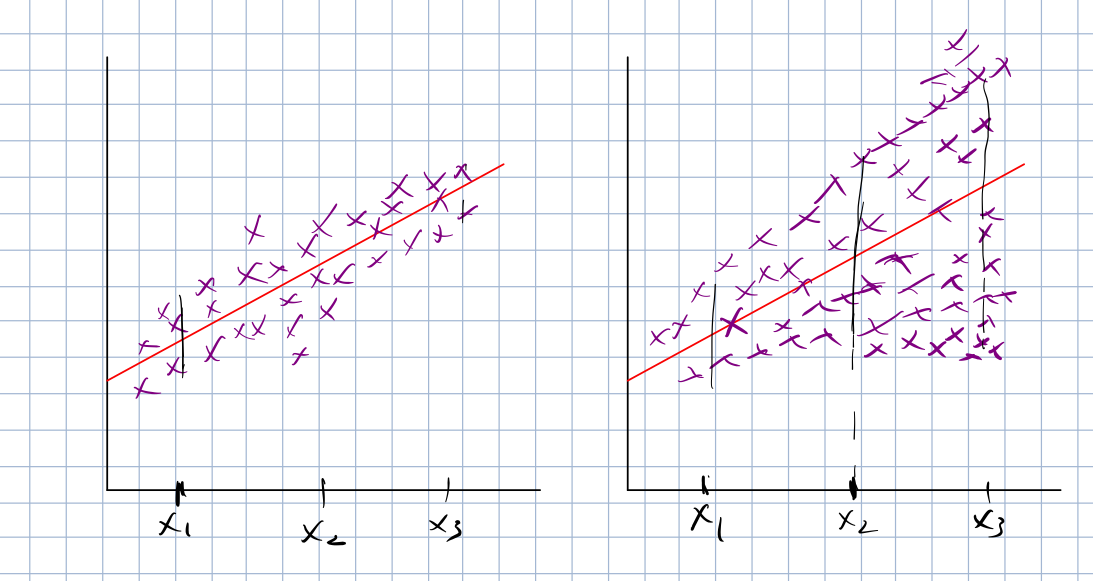
\includegraphics[width=0.55\textwidth]{hetero.png}
\end{figure}
\par\medskip
From the figure, we can see that the variance of the error term changes with $X_i$. In such case, standard errors of our estimators must take this into account. Running two versions of the regression in STATA would help. The homoskedastic version could be obtained by \texttt{regress y x}, while the heteroskedastic version requires \texttt{regress y x, vce(robust)} or \texttt{regress y x, robust}.  Below, I regressed the codes from the previous recitation for comparison. \par\medskip
\begin{figure}[H]
\centering
\begin{subfigure}[H]{0.475\textwidth}
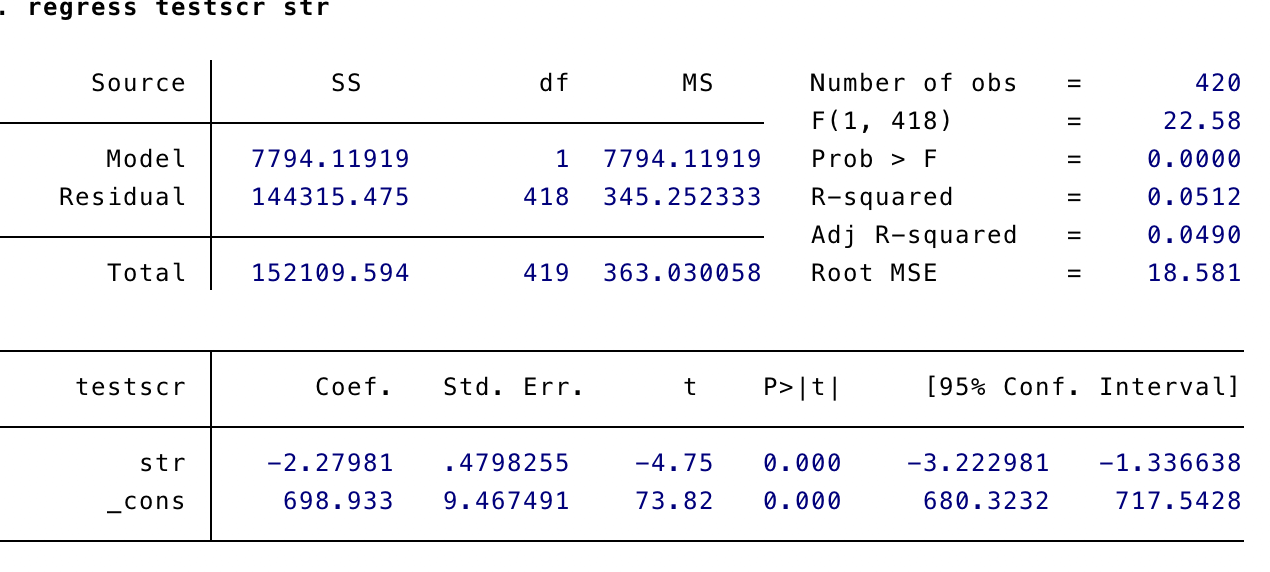
\includegraphics[width=\textwidth]{nonrobust.png}
\end{subfigure}
\begin{subfigure}[H]{0.475\textwidth}
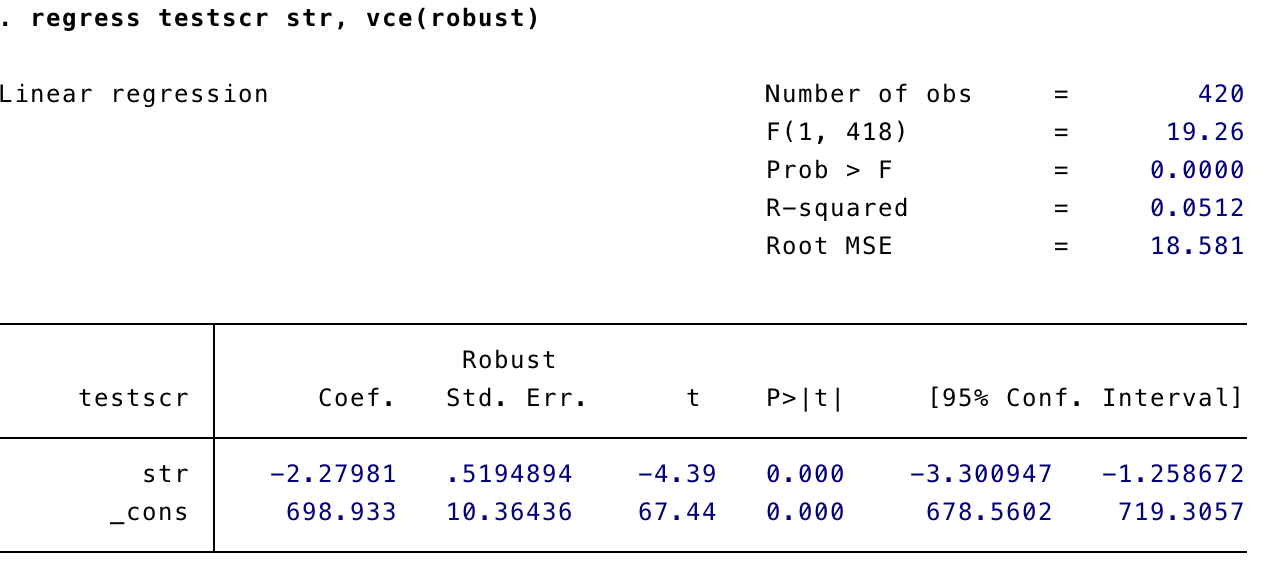
\includegraphics[width=\textwidth]{robust.png}
\end{subfigure}
\end{figure}
There are two takeaways from the picture
\begin{itemize}
\item \textbf{The variance rises (usually) in the heteroskedastic regression.} In other words, when we keep homoskedasticity assumption in cases where we should not do so, we end up rejecting null hypothesis that should not be rejected.
\item \textbf{The coefficients are unchanged.} When calculating the values for the estimators, we did not rely on the homoskedasticity assumption. Therefore, the coefficients are unaffected. In other words, the estimates are still unbiased.
\end{itemize}
%%%%%%%%%%%%%%%
\end{document}

